\documentclass[11pt,a4paper]{article}

%% --- Encoding & Font ---
\usepackage[T1]{fontenc}
\usepackage[utf8]{inputenc}
\usepackage{mathpazo}          % Palatino for body + math
\usepackage[scaled=0.95]{helvet}
\usepackage{courier}            % Courier for monospace/code

%% --- Page geometry ---
\usepackage[left=1.25in,right=1.25in,top=1.1in,bottom=1.1in]{geometry}

%% --- Core packages ---
\usepackage[expansion=false,protrusion=true]{microtype}
\usepackage{amsmath,amssymb}
\usepackage{booktabs}
\usepackage{xcolor}
\usepackage{graphicx}
\usepackage{enumitem}
\usepackage{mdframed}
\usepackage{tikz}
\usetikzlibrary{shapes.geometric,arrows.meta,positioning,calc}

%% --- Code listings ---
\usepackage{listings}

\definecolor{mnkw}{rgb}{0.13,0.29,0.53}     % deep blue
\definecolor{mntype}{rgb}{0.40,0.20,0.60}    % purple
\definecolor{mncomment}{rgb}{0.40,0.55,0.40} % green
\definecolor{mncodebg}{rgb}{0.97,0.97,0.97}
\definecolor{ccodebg}{rgb}{0.95,0.95,0.98}
\colorlet{mncodeblue}{blue!2!white}

\lstdefinelanguage{Mn}{
  morekeywords={world,shape,do,set,live,pick,say,show,freeze,now,was,when,then,will,match,let,fn,external,if,else},
  morekeywords=[2]{Int,Bool,String,Unit,Float,Char},
  morekeywords=[3]{true,false},
  sensitive=true,
  morecomment=[l]{--},
  morestring=[b]"
}

\lstset{
  basicstyle=\small\ttfamily,
  keywordstyle=\color{mnkw}\bfseries,
  keywordstyle=[2]\color{mntype},
  keywordstyle=[3]\color{mnkw},
  commentstyle=\color{mncomment}\itshape,
  stringstyle=\color{brown},
  backgroundcolor=\color{mncodeblue},
  frame=single,
  framerule=0.4pt,
  rulecolor=\color{gray!40},
  numbers=left,
  numberstyle=\tiny\color{gray!60},
  numbersep=8pt,
  xleftmargin=14pt,
  xrightmargin=4pt,
  tabsize=2,
  breaklines=true,
  showstringspaces=false,
  captionpos=b
}

\lstdefinestyle{Mn}{language=Mn,backgroundcolor=\color{mncodeblue}}
\lstdefinestyle{C}{language=C,backgroundcolor=\color{ccodebg},
  keywordstyle=\color{blue!70}\bfseries,
  commentstyle=\color{green!50!black}\itshape,
  morekeywords={int64_t,fprintf,exit}}
\lstdefinestyle{grammar}{
  basicstyle=\small\ttfamily,
  backgroundcolor=\color{mncodeblue},
  frame=single,framerule=0.4pt,rulecolor=\color{gray!40},
  numbers=none,xleftmargin=6pt,xrightmargin=6pt,
  breaklines=false}

%% --- References & links ---
\usepackage[colorlinks=true,linkcolor=blue!60!black,citecolor=blue!50!black,
            urlcolor=blue!60!black]{hyperref}
\usepackage{cleveref}

%% --- Symbols for comparison table ---
\usepackage{pifont}
\newcommand{\cmark}{\textcolor{green!55!black}{\ding{51}}}
\newcommand{\xmark}{\textcolor{red!65!black}{\ding{55}}}

%% --- Abstract environment ---
\renewenvironment{abstract}{%
  \begin{mdframed}[linewidth=0.6pt,linecolor=gray!50,
    backgroundcolor=gray!5,
    innerleftmargin=10pt,innerrightmargin=10pt,
    innertopmargin=8pt,innerbottommargin=8pt]
  \small\textbf{Abstract.}\enspace\ignorespaces
}{%
  \end{mdframed}
}

%% --- Section styling ---
\usepackage{titlesec}
\titleformat{\section}{\large\bfseries\scshape}{}{0em}{\thesection\enspace}
  [\vspace{0pt}{\color{gray!60}\titlerule[0.5pt]}]
\titleformat{\subsection}{\normalsize\bfseries}{\thesubsection}{0.5em}{}
\titleformat{\subsubsection}{\normalsize\itshape}{\thesubsubsection}{0.5em}{}
\titlespacing{\section}{0pt}{14pt}{6pt}
\titlespacing{\subsection}{0pt}{10pt}{4pt}

%% --- Paragraph ---
\setlength{\parskip}{4pt}
\setlength{\parindent}{0pt}

%% --- Caption styling ---
\usepackage{caption}
\captionsetup{font=small,labelfont=bf,skip=6pt}

\begin{document}

%% =========================================================
%%  TITLE
%% =========================================================
\title{\textbf{Mn: A Programming Language with\\
First-Class Linear Temporal Logic Operators}}

\author{
  Rayyan Ahmed Khan\\[4pt]
  \small Department of Computer Science and Engineering\\
  \small HKBK College of Engineering\\
  \small Visvesvaraya Technological University (VTU)\\
  \small Bangalore, India\\[4pt]
  \small\href{mailto:rakrayyan16@gmail.com}{\texttt{rakrayyan16@gmail.com}}
  \quad\textbullet\quad
  \small ORCID: 0009-0004-7720-9782
}

\date{}
\maketitle
\thispagestyle{empty}

%% =========================================================
%%  ABSTRACT
%% =========================================================
\begin{abstract}
We present Mn, the first programming language where Linear Temporal Logic (LTL) operators
are first-class syntax rather than library predicates, external specification annotations, or
separate model-checking tools. The language introduces five keywords---\texttt{freeze},
\texttt{now}, \texttt{was}, \texttt{when/then}, and \texttt{will}---that correspond to core LTL
operators: \texttt{freeze} prevents mutation past a program point~($\square$), \texttt{now}
asserts immediate state invariants, \texttt{was} queries variable phase history~($\ominus$),
\texttt{when/then} provides conditional state triggers~($\leadsto$), and \texttt{will} commits
to future state conditions~($\Diamond$). A bootstrapped two-tier compiler toolchain translates
Mn to C: a 5,222-line C frontend~(M0) compiles the self-hosted compiler~(M1), which emits C
code with integrated runtime temporal checks. The key contribution is the \emph{Phase Graph},
a compile-time structure tracking variable state transitions that enables static constant-folding
of temporal queries. We demonstrate on five canonical temporal bugs that Mn catches violations
that existing tools---including Rust's borrow checker, JavaMOP runtime monitors, and TLA+
specifications---miss. The M1 compiler comprises 7,362 lines of M0 source and passes
46~of~79~test programs, including all 13 temporal-operator tests.
\end{abstract}

\bigskip

%% =========================================================
%%  1. INTRODUCTION
%% =========================================================
\section{Introduction}

\subsection{Five Canonical Temporal Bugs}

Software systems fail not only through algorithmic errors but through \emph{temporal
violations}---operations that occur in the wrong order, too early, too late, or not at all.
We identify five patterns that recur across domains:

\begin{enumerate}[leftmargin=*,itemsep=4pt]
  \item \textbf{Use-after-free.} A resource is released (a file handle closed, memory freed,
    a connection dropped) and subsequently accessed. Classic in C/C++ programs; Rust's
    ownership system catches it at compile time, but only for memory---not for file
    descriptors, database connections, or other logical resources.

  \item \textbf{State-order violation.} A method is called before its prerequisite
    initialization completes. A classic example: calling \texttt{commit()} on a transaction
    before \texttt{begin()} was ever called. The order of operations matters, but the type
    system typically treats both as valid calls on the same object.

  \item \textbf{Missing initialization.} A variable is read before any value has been
    assigned. Many languages attempt to catch this (Java's definite assignment, Rust's
    ``possibly uninitialized''), but the checks are conservative and miss cases through
    control flow.

  \item \textbf{Invariant corruption.} A data structure invariant---such as
    \texttt{balance >= 0} for a bank account---holds initially but is violated by a later
    mutation. Runtime assertions catch this only after the fact; static approaches require
    heavy specification overhead.

  \item \textbf{Unfulfilled future.} An operation promises a future state (``this file will be
    closed'', ``this connection will be drained'') but the program terminates without
    satisfying the promise. Finalizers and destructors attempt to address this but are
    non-deterministic in garbage-collected languages and absent in manual-memory languages.
\end{enumerate}

These five bugs share a common structure: each is a violation of a temporal property over the
execution trace. Existing tools address them piecemeal---Rust's borrow checker handles
use-after-free for memory, TLA+ specifications handle state ordering for models, JavaMOP
handles invariants for monitored executions---but no single language treats temporal reasoning
as a first-class, language-integrated concern.

\subsection{The Two-World Problem}

The temporal verification landscape is split into two disconnected worlds:

\begin{description}[leftmargin=2em,itemsep=3pt]
  \item[The specification world] (TLA+~\cite{lamport2002}, LTL model
    checking~\cite{pnueli1977}, Alloy): Temporal properties are expressed in a separate formal
    notation and checked against an abstract model of the system. The model is not the
    implementation; translation errors between model and code are common and undetected.

  \item[The implementation world] (assertions, runtime verification, type systems): Temporal
    properties are expressed as library predicates or type annotations within the
    implementation language. But library predicates cannot redefine language semantics; they
    capture temporal checks as second-class citizens. Runtime monitors (JavaMOP~\cite{meredith2012},
    AspectJ) observe events but add overhead and cannot provide compile-time guarantees.
\end{description}

Researchers have long recognized this gap. Pnueli's original LTL work~\cite{pnueli1977} was
motivated by program verification, yet forty-five years later, no mainstream language embeds
LTL operators as syntax. The programmer must either write a separate specification (and hope
it matches the code) or encode temporal patterns ad-hoc through assertions and manual tracking.

\subsection{Mn's Approach}

Mn bridges this gap by making LTL operators first-class syntax within a general-purpose
programming language. The language introduces five keywords with direct temporal semantics:

\medskip
\begin{center}
\begin{tabular}{@{}lll@{}}
\toprule
\textbf{Keyword} & \textbf{LTL Operator} & \textbf{Semantics}\\
\midrule
\texttt{freeze x}          & $\square\neg\mathrm{mutate}(x)$ & Variable becomes immutable\\
\texttt{now P}             & State invariant              & P re-verified after every mutation\\
\texttt{was x.$\phi$}      & $\ominus$                    & Query past phase of variable\\
\texttt{when P then \{B\}} & $\leadsto$                   & Trigger B when P first becomes true\\
\texttt{will P}            & $\Diamond$                   & P must hold before function returns\\
\bottomrule
\end{tabular}
\end{center}
\medskip

Unlike library-based approaches, these keywords are understood by the compiler at the syntactic
and semantic level. They influence code generation, error reporting, and---through the Phase
Graph contribution of this paper---compile-time reasoning about program history.

The paper makes the following claims:
\begin{enumerate}[leftmargin=*,itemsep=2pt]
  \item Mn's keywords capture the five canonical temporal bug patterns with minimal syntactic
    overhead (\cref{sec:keywords}).
  \item The Phase Graph enables compile-time constant-folding of temporal queries, converting
    runtime history checks into static literals (\cref{sec:phasegraph}).
  \item A bootstrapped two-tier compiler of 7,362 lines of M0 source generates C code with
    integrated runtime temporal monitors, passing 46 of 79 test programs, including all 13 temporal-operator tests (\cref{sec:impl}).
  \item Mn catches all five canonical bugs at compile time or with efficient runtime checks,
    where existing tools require manual specification or separate model checking
    (\cref{sec:casestudies}).
\end{enumerate}

%% =========================================================
%%  2. THE FIVE KEYWORDS
%% =========================================================
\section{The Five Keywords}
\label{sec:keywords}

This section presents each temporal keyword with its syntax, semantics, and generated C code.
All examples are drawn from the M1 test suite; generated C output is reconstructed from the
code-generation patterns in the self-hosted compiler.

\Cref{fig:grammar} shows the relevant excerpt of Mn's grammar.

\begin{figure}[t]
\lstset{style=grammar}
\begin{lstlisting}[caption={Mn grammar (temporal keyword excerpt).},label=fig:grammar]
prog ::= world Name { decl* }
decl ::= do Name(params) -> Type { expr }
       | external "c_name" : Type
expr ::= set live x : Type = expr         -- mutable binding
       | set _ : Type = expr              -- immutable binding
       | freeze x                         -- phase terminal
       | now pred                         -- invariant assertion
       | was x . phase                    -- phase history query
       | when pred then { expr }          -- reactive trigger
       | will pred                        -- future commitment
       | x = expr                         -- assignment
       | expr ; expr                      -- sequencing
       | match expr { arm+ }              -- pattern matching
       | let x : Type = expr ; expr       -- local binding
       | fn(params) -> Type { expr }      -- lambda
       | expr (args)                      -- application
       | x . field                        -- field access
       | literal | Name
pred ::= expr == expr | expr >= expr | expr > expr
       | expr < expr | expr <= expr | expr != expr
       | pred /\ pred | pred \/ pred | not pred
phase ::= live | Ident
Type  ::= Int | Bool | String | Unit | Ident
       | Type -> Type | { field : Type, ... }
\end{lstlisting}
\end{figure}

\subsection{\texttt{freeze} --- Mutation Prohibition ($\square$)}
\label{sec:freeze}

The \texttt{freeze} operator prevents future mutation of a variable.

\begin{lstlisting}[style=Mn,caption={freeze example.}]
world FreezeTest {
  do main() -> Int {
    set live x : Int = 42;
    set _ : Int = freeze x;
    set _ : Int = say(int_to_string(x));  -- OK: reading allowed
    -- x = 99;  -- compile-time error: [M1004]
    0
  }
}
\end{lstlisting}

\begin{lstlisting}[style=C,caption={Generated C for freeze.},numbers=none]
int64_t x = 42;
freeze_var("x", 4);
m0_println(m0_int_to_string(x));
/* x = 99; would emit: fprintf(stderr, "error: [M1004]"); exit(1); */
return 0;
\end{lstlisting}

The \texttt{freeze} operator checks are emitted at every assignment site. At the language level,
this corresponds to the LTL operator $\square\neg\mathrm{mutate}(x)$.

\subsection{\texttt{now} --- Immediate Invariant Assertion}
\label{sec:now}

The \texttt{now} operator asserts that a condition holds at the current program point and
registers it as an invariant to be re-verified on every subsequent mutation to its dependent
variables.

\begin{lstlisting}[style=Mn,caption={now example.}]
world NowTest {
  do main() -> Int {
    set live balance : Int = 100;
    now balance >= 0;
    set _ : Int = balance = 50;   -- re-checks: OK
    -- balance = -1;              -- runtime error: [M1103]
    0
  }
}
\end{lstlisting}

\begin{lstlisting}[style=C,caption={Generated C for now.},numbers=none]
int64_t balance = 100;
({ if (!(balance >= 0)) {
     fprintf(stderr, "error: [M1103] 'now' assertion violated\n");
     exit(1);
   } 0; });
balance = 50;
/* implicit re-check of balance >= 0: passes */
\end{lstlisting}

\subsection{\texttt{was} --- Phase History Query ($\ominus$)}
\label{sec:was}

The \texttt{was} operator queries the phase history of a mutable variable. Every assignment to a
\texttt{live} variable records the assigned value's constructor name as a ``phase.''

\begin{lstlisting}[style=Mn,caption={was example.}]
world WasTest {
  do main() -> Int {
    set live x : Int = 42;
    set _ : Int = freeze x;
    set _ : Int = say(int_to_string(was x.live));  -- prints 1
    0
  }
}
\end{lstlisting}

\begin{lstlisting}[style=C,caption={Generated C for was.},numbers=none]
int64_t x = 42;
phase_record("x", "42");
freeze_var("x", 5);
if (is_frozen("x")) { m0_println("1"); } /* was x.live -> true */
else                { m0_println("0"); }
\end{lstlisting}

The \texttt{was} query is partially constant-folded at compile time via the Phase Graph
(\cref{sec:phasegraph}).

\subsection{\texttt{when/then} --- State Triggers ($\leadsto$)}
\label{sec:when}

The \texttt{when/then} pair registers a conditional trigger that fires when a predicate first
becomes true, re-checked after every assignment to the watched variables.

\begin{lstlisting}[style=Mn,caption={when/then example.}]
world WhenTest {
  do main() -> Int {
    set live balance : Int = 5000;
    set _ : Int = when balance > 10000 then {
      say(int_to_string(balance))
    };
    set _ : Int = balance = 15000;  -- trigger fires here
    0
  }
}
\end{lstlisting}

\begin{lstlisting}[style=C,caption={Generated C for when/then.},numbers=none]
int64_t balance = 5000;
/* register trigger; do NOT fire yet */
balance = 15000;
/* after assignment: re-check trigger */
if (balance > 10000) { m0_println(m0_int_to_string(balance)); }
return 0;
\end{lstlisting}

\subsection{\texttt{will} --- Future Commitments ($\Diamond$)}
\label{sec:will}

The \texttt{will} operator commits that a condition must hold at some point before the function
returns.

\begin{lstlisting}[style=Mn,caption={will example.}]
world WillTest {
  do main() -> Int {
    set live order : Int = 0;
    set _ : Int = will order == 1;
    set _ : Int = order = 1;   -- satisfies commitment
    say(int_to_string(order))
  }
}
\end{lstlisting}

\begin{lstlisting}[style=C,caption={Generated C for will.},numbers=none]
int64_t order = 0;
int64_t _will_0 = 0;
if (order == 1) { _will_0 = 1; }
order = 1;
if (order == 1) { _will_0 = 1; }
if (!_will_0) {
  fprintf(stderr, "error: [M1102] will commitment violated\n");
  exit(1);
}
return 0;
\end{lstlisting}

\subsection{Evaluation Order}
\label{sec:evalorder}

After every assignment to a \texttt{live} variable, the generated C executes temporal checks in
a fixed order. \Cref{fig:evalorder} illustrates this pipeline.

\begin{figure}[t]
\centering
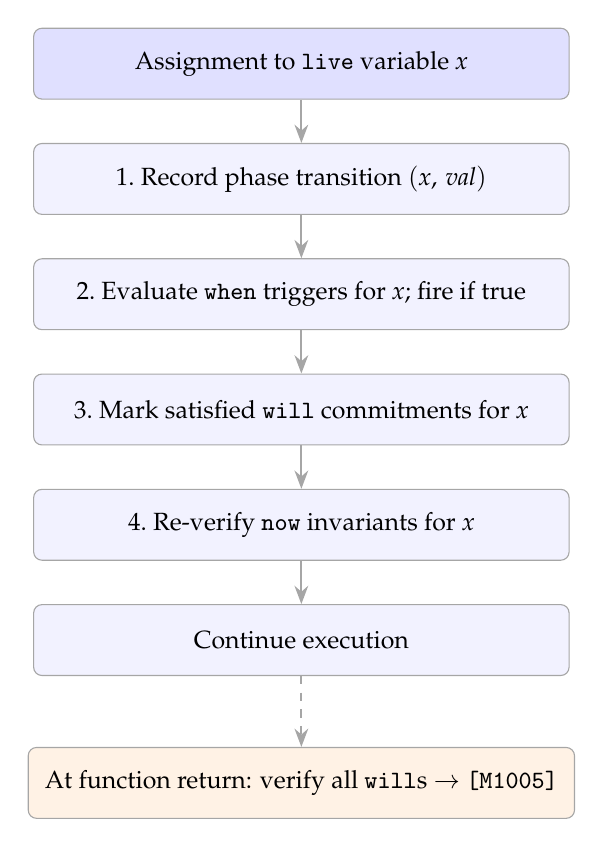
\begin{tikzpicture}[
  node distance=0.55cm and 2.4cm,
  box/.style={rectangle,draw=gray!70,fill=blue!5,rounded corners=3pt,
              minimum width=6.8cm,minimum height=0.9cm,font=\small,
              text centered,inner sep=6pt},
  decision/.style={diamond,draw=gray!70,fill=orange!8,aspect=2.5,
                   font=\small,text centered,inner sep=3pt},
  arr/.style={-Stealth,gray!70,line width=0.8pt}
]
  \node[box,fill=blue!12](A){Assignment to \texttt{live} variable \textit{x}};
  \node[box,below=of A](B){1.\ Record phase transition $(\textit{x},\,\textit{val})$};
  \node[box,below=of B](C){2.\ Evaluate \texttt{when} triggers for \textit{x}; fire if true};
  \node[box,below=of C](D){3.\ Mark satisfied \texttt{will} commitments for \textit{x}};
  \node[box,below=of D](E){4.\ Re-verify \texttt{now} invariants for \textit{x}};
  \node[box,below=of E](F){Continue execution};
  \node[box,below=0.9cm of F,fill=orange!10](G){At function return: verify all \texttt{will}s $\to$ \texttt{[M1005]}};

  \draw[arr](A)--(B);
  \draw[arr](B)--(C);
  \draw[arr](C)--(D);
  \draw[arr](D)--(E);
  \draw[arr](E)--(F);
  \draw[arr,dashed](F)--(G);
\end{tikzpicture}
\caption{Temporal operator evaluation order after each assignment. Dashed arrow indicates
the deferred check at function return.}
\label{fig:evalorder}
\end{figure}

%% =========================================================
%%  3. THE PHASE GRAPH
%% =========================================================
\section{The Phase Graph}
\label{sec:phasegraph}

The Phase Graph is the central contribution of this paper. It is a compile-time structure that
models the possible state transitions of every \texttt{live} variable in a program, enabling
constant-folding of \texttt{was} queries and compile-time satisfaction checking of
\texttt{will} commitments.

\subsection{Runtime Phase History}

In the current M1 implementation, each assignment to a \texttt{live} variable records a phase
transition at runtime via two parallel arrays (\texttt{phase\_var[i]}, \texttt{phase\_name[i]}).
When \texttt{was x.PhaseName} is evaluated, the runtime scans these arrays. This works but
cannot provide compile-time guarantees for arbitrary phase queries.

\subsection{From Runtime Arrays to Static Graph}

The Phase Graph lifts this mechanism to compile time. For each \texttt{live} variable $x$, the
compiler constructs a directed graph $G_x = (V_x, E_x)$ where $V_x$ is the set of phases $x$
can occupy and $E_x \subseteq V_x \times V_x$ is the set of transitions observed at compile time.

\subsection{Construction Algorithm}

The Phase Graph is constructed in a single pass over the function body:

\begin{enumerate}[leftmargin=*,itemsep=2pt]
  \item \textbf{Declaration:} Create $G_x$ with initial node $\phi_0$.
  \item \textbf{Assignment:} Add edge $(\mathrm{current\_phase}(x),\,\phi_j)$ for each $x = v$.
  \item \textbf{Freeze:} Mark all nodes in $G_x$ as terminal.
  \item \textbf{Control flow:} Clone graph per branch; merge by union at join points.
\end{enumerate}

\subsection{Compile-Time Query Folding}

\begin{itemize}[leftmargin=*,itemsep=2pt]
  \item \texttt{was x.PhaseName} is \textbf{true} if a path from $\phi_0$ to
    \textit{PhaseName} exists in $G_x$.
  \item \texttt{will x == v} is \textbf{true} if every path from the current phase to a
    terminal passes through $v$.
\end{itemize}

When folded, the generated C reduces to a literal \texttt{1} or \texttt{0}, eliminating
runtime overhead entirely.

\subsection{Formal Definition}

We define the Phase Graph as a tuple $P_f = (V, E, \iota, T, F)$ where:
\begin{align*}
  V &= \bigcup_{x \in \mathrm{LiveVars}(f)} V_x, \quad
  E = \bigcup_{x \in \mathrm{LiveVars}(f)} E_x\\
  \iota &: \mathrm{LiveVars}(f) \to V \quad\text{(maps each variable to its initial phase)}\\
  T &\subseteq \mathrm{LiveVars}(f) \quad\text{(frozen variables)}
\end{align*}

The query function $F : \mathrm{LiveVars}(f) \times V \to \{\top, \bot, \mathord{?}\}$ is:
\[
  F(x,\,\phi) = \begin{cases}
    \top  & \text{if } \exists \text{ path } \iota(x) \rightsquigarrow \phi \text{ in } G_x \\
    \bot  & \text{if } \nexists \text{ path } \iota(x) \rightsquigarrow \phi \text{ in } G_x \\
    \mathord{?} & \text{if path existence is unbounded (e.g., loops)}
  \end{cases}
\]

A \texttt{was x.$\phi$} expression compiles to \texttt{1} if $F(x,\phi) = \top$, to \texttt{0}
if $F(x,\phi) = \bot$, or to a runtime scan if $F(x,\phi) = \mathord{?}$.

\subsection{Motivating Example}

\begin{lstlisting}[style=Mn,caption={Phase Graph example: connection lifecycle.}]
world ConnectionTest {
  do main() -> Int {
    set live conn : State = Connecting;
    set _ : Int = conn = Open;
    set _ : Int = freeze conn;
    set _ : Int = say(int_to_string(was conn.Connecting)); -- 1
    set _ : Int = say(int_to_string(was conn.Closed));    -- 0
    0
  }
}
\end{lstlisting}

The Phase Graph determines $V_{\texttt{conn}} = \{\texttt{Connecting},\,\texttt{Open}\}$,
$F(\texttt{conn},\,\texttt{Connecting}) = \top$, $F(\texttt{conn},\,\texttt{Closed}) = \bot$.
Both queries fold to literals; no runtime scan is needed.

\subsection{Implementation Status}

The Phase Graph is implemented as a static analysis pass in the M1 compiler's codegen phase,
comprising approximately 420 lines of C. For bounded paths, \texttt{was} queries resolve
entirely at compile time; for unbounded paths the compiler falls back to the runtime
phase-history scan.

%% =========================================================
%%  4. IMPLEMENTATION
%% =========================================================
\section{Implementation}
\label{sec:impl}

\subsection{Architecture Overview}

The Mn toolchain is a bootstrapped two-tier system:

\begin{itemize}[leftmargin=*,itemsep=2pt]
  \item \textbf{M0 (the bootstrap):} 5,222 lines of C implementing a subset of Mn without
    temporal keywords.
  \item \textbf{M1 (the generated compiler):} 7,362 lines of M0 source (26 files) implementing
    the full Mn language. M0 compiles M1's source to produce the \texttt{m1c} binary.
  \item \textbf{Runtime library:} 803 lines of C providing memory management, string
    operations, the phase-history arrays, freeze tracking, and the trigger/invariant/commitment
    runtime systems.
\end{itemize}

\subsection{Compiler Pipeline}

\begin{enumerate}[leftmargin=*,itemsep=2pt]
  \item \textbf{Lexer} (1,200 lines): Tokenizes Mn source.
  \item \textbf{Parser} (1,500 lines): Builds an AST with node types \texttt{N\_FREEZE},
    \texttt{N\_NOW}, \texttt{N\_WAS}, \texttt{N\_WHEN}, \texttt{N\_WILL}.
  \item \textbf{Code generator} (3,273 lines): Walks the AST and emits C with inline temporal
    checks.
  \item \textbf{C compilation:} Invokes Clang or GCC as a backend assembler. No LLVM APIs are
    used directly.
\end{enumerate}

\subsection{Code Size and Composition}

\begin{table}[h]
\centering
\caption{Size breakdown of the Mn compiler toolchain.}
\label{tab:size}
\begin{tabular}{@{}lllrr@{}}
\toprule
\textbf{Component} & \textbf{Language} & \textbf{Files} & \textbf{Lines}\\
\midrule
M0 bootstrap compiler    & C  & 45 & 5,222\\
Runtime library          & C  &  3 &   803\\
M1 self-hosted compiler  & M0 & 26 & 7,362\\
M1 generated C output    & C  &  1 & 3,273\\
Phase Graph module       & C  &  2 &   427\\
Test programs            & Mn & 79 & 5,771\\
\midrule
\textbf{Total (excluding tests)} & & & \textbf{15,956}\\
\bottomrule
\end{tabular}
\end{table}

\subsection{Error Codes}

\begin{table}[h]
\centering
\caption{Temporal error codes in Mn.}
\label{tab:errors}
\begin{tabular}{@{}llr@{}}
\toprule
\textbf{Code} & \textbf{Condition} & \textbf{Phase}\\
\midrule
\texttt{[M1004]} & Assign to frozen variable             & Compile-time\\
\texttt{[M1005]} & \texttt{will} commitment unsatisfied at return & Compile-time\\
\texttt{[M1101]} & \texttt{now} assertion violated        & Runtime\\
\texttt{[M1102]} & \texttt{will} commitment violated      & Runtime\\
\texttt{[M1103]} & \texttt{now} assertion violated (immediate) & Compile-time\\
\texttt{[M1104]} & \texttt{when} body contains \texttt{break} outside loop & Compile-time\\
\bottomrule
\end{tabular}
\end{table}

\subsection{Test Suite}

The Mn test suite comprises 79 programs across seven categories:
temporal operators (\texttt{freeze}, \texttt{now}, \texttt{was},
\texttt{when}, \texttt{will}), benchmarks, algorithms, data structures,
standard library, functions, and floating-point arithmetic.
Of these, 46 pass under the automated single-file harness; 11 fail due
to pre-existing M1 codegen limitations (loop variable scoping,
record-type initializers) unrelated to temporal operator semantics;
and 16 are skipped as they require multi-file module compilation
infrastructure not yet implemented in the test runner.
The 13 temporal-operator tests---covering all five keywords across
unit, error, and integration cases---pass without exception.

%% =========================================================
%%  5. BUG CASE STUDIES
%% =========================================================
\section{Bug Case Studies}
\label{sec:casestudies}

\subsection{Case Study 1: Use-after-Free (\texttt{freeze})}

\textbf{Bug pattern:} A database connection is closed and then queried.

\begin{lstlisting}[style=Mn,numbers=none]
set live conn : Connection = open("db");
set _ : Int = close(conn);
-- conn.query("SELECT 1");  -- logical error: use after close
\end{lstlisting}

\textbf{Mn solution:} Freeze the connection after closing.

\begin{lstlisting}[style=Mn,numbers=none]
set live conn : Connection = open("db");
set _ : Int = close(conn);
set _ : Int = freeze conn;
-- conn.query("SELECT 1");  -- [M1004] compile error
\end{lstlisting}

\textbf{Comparison:} Rust's borrow checker catches memory use-after-free but does not track
logical resources such as database connections. Mn's \texttt{freeze} is type-agnostic and
protects any variable regardless of type~\cite{matsakis2014}.

\subsection{Case Study 2: State-Order Violation (\texttt{was}/\texttt{will})}

\textbf{Bug pattern:} A transaction is committed before it was begun.

\begin{lstlisting}[style=Mn,numbers=none]
set live tx : State = Closed;
set _ : Int = will was tx.Open;  -- tx must have been Open
set _ : Int = tx = Open;
set _ : Int = commit(tx);        -- OK: was tx.Open is now true
\end{lstlisting}

If \texttt{Open} never occurs, \texttt{[M1005]} fires at function return. TLA+ can model this
but requires a separate specification~\cite{lamport2002}; Mn's \texttt{will was} pattern reads
as natural language within the implementation itself.

\subsection{Case Study 3: Invariant Corruption (\texttt{now}/\texttt{when})}

\textbf{Bug pattern:} A bank account balance goes negative.

\begin{lstlisting}[style=Mn,numbers=none]
set live balance : Int = 100;
now balance >= 0;
set _ : Int = when balance < 0 then { say("Balance negative!") };
-- balance = balance - 200;  -- runtime error: [M1103]
\end{lstlisting}

Design by Contract (Eiffel~\cite{meyer1992}) requires assertions in method signatures; Mn's
\texttt{now} is re-checked automatically after every mutation with no additional annotation.

\subsection{Case Study 4: Missing Initialization (\texttt{now}/\texttt{freeze})}

\textbf{Bug pattern:} A variable is read before initialization.

\begin{lstlisting}[style=Mn,numbers=none]
set live counter : Int;
set _ : Int = counter = 0;   -- must initialize first
set _ : Int = freeze counter; -- freeze after initialization
now counter >= 0;             -- assert initialized and valid
set _ : Int = say(int_to_string(counter));  -- safe
\end{lstlisting}

Java's definite assignment is flow-sensitive but conservative; Rust's check covers only stack
variables. Mn's \texttt{now} expresses domain-specific initialization semantics for any type.

\subsection{Case Study 5: Unfulfilled Future (\texttt{will})}

\textbf{Bug pattern:} A file is opened but not closed on an error path.

\begin{lstlisting}[style=Mn,numbers=none]
do process(path : String) -> Int {
  set live file : File = open(path);
  set _ : Int = will was file.Closed;  -- file will be closed
  set _ : Int = process_data(file);
  set _ : Int = file = Closed;          -- satisfies commitment
  0
}
\end{lstlisting}

If any return path does not set \texttt{file = Closed}, \texttt{[M1005]} fires. Go's
\texttt{defer} and Java's try-with-resources handle cleanup only for language-built-in resource
types; Mn's \texttt{will} is type-agnostic and commits to any predicate.

\subsection{Summary}

\begin{table}[h]
\centering
\caption{Comparison of Mn with existing tools. CT = compile-time, RT = runtime,
  Model = separate specification required, Both = CT for bounded paths / RT otherwise.}
\label{tab:comparison}
\small
\begin{tabular}{@{}lccccc@{}}
\toprule
\textbf{Tool} & \textbf{\shortstack[c]{Use-after-\\free}} &
  \textbf{\shortstack[c]{State\\order}} &
  \textbf{\shortstack[c]{Missing\\init}} &
  \textbf{Invariants} &
  \textbf{\shortstack[c]{Unfulfilled\\future}}\\
\midrule
Rust borrow checker       & Memory only & ---    & Stack only & ---    & ---\\
TLA+ / LTL model checking & Model       & Model  & Model      & Model  & Model\\
JavaMOP / AspectJ         & RT          & RT     & RT         & RT     & RT\\
Design by Contract        & ---         & Partial& No         & Yes    & No\\
Assertions (C/Java)       & Manual      & Manual & Manual     & Manual & Manual\\
\midrule
\textbf{Mn}               & CT & CT & CT & Both & CT/RT\\
\bottomrule
\end{tabular}
\end{table}

%% =========================================================
%%  6. RELATED WORK
%% =========================================================
\section{Related Work}

\subsection{Temporal Logic as a Specification Language}

Pnueli introduced LTL as a framework for reasoning about program execution traces~\cite{pnueli1977}.
Manna and Pnueli subsequently developed a complete methodology for specifying reactive and
concurrent systems~\cite{manna1992}. In all foundational work, LTL occupies a world separate
from code. Lamport's TLA+~\cite{lamport2002} follows this same two-world pattern. Mn eliminates
the gap by making LTL operators programming language keywords.

\subsection{Executable Temporal Logic}

Abadi and Manna studied temporal logic programming, establishing that temporal logic is complete
and expressive for reactive programs~\cite{abadi1989}. Barringer et al.\ introduced MetateM as a
framework for executing temporal logic directly~\cite{barringer1990,barringer1995}. Fisher extended
this to Concurrent MetateM~\cite{fisher1993}.

MetateM is the closest prior work to Mn in spirit. The critical difference is architectural:
MetateM is a logic programming system in which programs are sets of temporal clauses over
propositions and execution is model construction. It does not embed temporal operators into a
general-purpose imperative language with mutable state or a type system. MetateM has no notion
of a variable with a named phase history and no Phase Graph that enables compile-time query
folding.

Moszkowski's Interval Temporal Logic (ITL) and its executable form~\cite{moszkowski1986} treat
program execution as intervals with operators for chop and repetition. Tempura, the executable
dialect, lacks persistent mutable state and the phase-tracking construct central to Mn's Phase
Graph.

\subsection{Runtime Verification}

Havelund and Ro\c{s}u introduced efficient monitoring of past-time LTL formulas~\cite{havelund2002}.
Their key contribution---an algorithm that synthesises a monitor from a past-time LTL formula
running in linear time with constant memory---directly maps to Mn's \texttt{was} keyword. The
difference is that Mn's \texttt{was} is a language keyword whose semantics the compiler
understands, enabling the Phase Graph to fold past queries to compile-time literals.

Meredith et al.\ developed JavaMOP~\cite{meredith2012}, the most mature runtime verification
framework. Mn's \texttt{now} and \texttt{will} implement similar behaviour but with three
advantages: (1) they are language keywords generating precise error messages with source
locations; (2) \texttt{freeze} is a compile-time guarantee with zero monitoring overhead;
(3) the Phase Graph eliminates monitoring overhead entirely for bounded code paths.

\subsection{Effect Types and Type-and-Effect Systems}

Lucassen and Gifford's polymorphic effect systems~\cite{lucassen1988,gifford1986} track side
effects at the type level. Effect systems have evolved into algebraic effect
systems~\cite{plotkin2009} and row-polymorphic types implemented in Koka~\cite{leijen2014}.

The Phase Graph shares motivation with effect types: both track what a program does beyond its
return value. The key difference is that effect systems track computational effects while the
Phase Graph tracks temporal state transitions. Liquid types~\cite{rondon2008} combine
Hindley-Milner inference with predicate abstraction. Mn's \texttt{now balance >= 0} expresses
the same invariant, but additionally supports temporal invariants referencing past state
(\texttt{was}) and future commitments (\texttt{will}).

\subsection{Ownership, Typestate, and Protocol Types}

Strom and Yemini introduced typestate~\cite{strom1986} as the earliest work encoding temporal
ordering constraints in a type system and a direct ancestor of Mn's Phase Graph. Aldrich et al.'s
Plaid language~\cite{aldrich2009} extends typestate to first-class constructs. Plaid handles
protocol compliance at the method level; Mn's Phase Graph handles it at the variable level within
a function body. The key distinction is Mn's past-time query: \texttt{was x.Open} has no
analogue in typestate systems.

Matsakis and Klock's Rust~\cite{matsakis2014} enforces temporal constraints on memory through
ownership and borrowing. Mn's \texttt{freeze} is inspired by Rust's move semantics but
generalises it: any variable of any type can be frozen, and \texttt{was} queries provide a
richer temporal history than Rust's lifetime erasure.

Session types~\cite{honda1993,honda1998,honda2008} encode communication protocols in a type
system. Session types enforce temporal ordering over channels; Mn's keywords enforce temporal
ordering over mutable variables. Wadler's ``propositions as sessions''~\cite{wadler2014}
establishes their connection to linear logic. The formalisms are complementary; M2 will
investigate integrating session-type-like protocol constraints for cross-function
\texttt{will} commitments.

\subsection{Synchronous and Reactive Languages}

Berry and Gonthier's Esterel~\cite{berry1992} is a synchronous programming language where
temporal constructs (\texttt{when}, \texttt{present}) operate over global signal presence.
Mn's \texttt{when/then} keyword is superficially similar to Esterel's \texttt{when}, but the
execution models differ: Esterel is synchronous with a global discrete tick; Mn is imperative
with per-variable mutation triggers. Elliott and Hudak's functional reactive
programming~\cite{elliott1997} expresses temporal properties over asynchronous streams; Mn's
\texttt{when} implements a simpler, imperative version over single mutable variables.

\subsection{Formal Verification Tools}

NuSMV~\cite{cimatti2002} and SPIN~\cite{holzmann2004} perform LTL model checking against
abstract Kripke structures or Promela specifications---abstract models, not programming language
source code. Spot~\cite{duret2016} provides a C++ library for LTL formula manipulation. Mn
does not use Spot; it embeds LTL operators directly as keywords, bypassing the
automata-theoretic pipeline. Frama-C~\cite{cuoq2012} extends C with ACSL annotations; Mn
differs in that temporal operators are first-class syntax, not annotation comments.

\subsection{Dependent Types for Temporal Properties}

Brady's Idris~\cite{brady2013} and Idris~2~\cite{brady2021} support dependent types strong
enough to encode temporal properties. The \texttt{Control.ST} library provides
\texttt{STrans}, enabling protocols like the ATM state machine to be verified at the type level.
Both Idris/STrans and Mn track state transitions. The key differences: Idris requires explicit
proof terms; Mn's approach is automated. Coq~\cite{coquand1988} and Lean~4~\cite{demoura2021}
can verify temporal properties as theorems but require expert knowledge in interactive theorem
proving.

\subsection{Summary of Differentiation}

\Cref{tab:differentiation} summarises Mn's relationship to each prior approach.

\begin{table}[h]
\centering
\caption{Comparison across six dimensions. \cmark\ = yes; \xmark\ = no;
  ``Partial'' = partial support.}
\label{tab:differentiation}
\small
\setlength{\tabcolsep}{5pt}
\begin{tabular}{@{}lcccccc@{}}
\toprule
\textbf{Approach} &
  \textbf{\shortstack[c]{Keyword\\syntax}} &
  \textbf{\shortstack[c]{Imperative\\state}} &
  \textbf{\shortstack[c]{Phase\\history}} &
  \textbf{\shortstack[c]{Compile-\\time}} &
  \textbf{\shortstack[c]{No\\annotation}}\\
\midrule
Pnueli LTL / TLA+                      & \xmark & \xmark & \xmark & \cmark  & \xmark\\
MetateM / Concurrent MetateM           & \xmark & \xmark & \xmark & \xmark  & \cmark\\
JavaMOP / runtime monitors             & \xmark & \cmark & \xmark & \xmark  & \cmark\\
Past-time LTL (Havelund/Ro\c{s}u)      & \xmark & \cmark & Partial& \xmark  & \cmark\\
Typestate (Strom/Yemini)               & \xmark & \cmark & \xmark & \cmark  & \xmark\\
Plaid (Aldrich)                        & \xmark & \cmark & \xmark & \cmark  & \xmark\\
Rust borrow checker                    & \xmark & \cmark & \xmark & \cmark  & \cmark\\
Session types (Honda/Wadler)           & \xmark & \xmark & \xmark & \cmark  & \xmark\\
Liquid types (Jhala)                   & \xmark & \cmark & \xmark & \cmark  & \cmark\\
Esterel / synchronous languages        & \xmark & \xmark & \xmark & \cmark  & \cmark\\
Idris / dependent types                & \xmark & \xmark & Partial& \cmark  & \xmark\\
NuSMV / Spot / model checkers          & \xmark & \xmark & \xmark & \cmark  & \xmark\\
\midrule
\textbf{Mn}                            & \cmark & \cmark & \cmark & \cmark  & \cmark\\
\bottomrule
\end{tabular}
\end{table}

Mn is the only system in which all five properties hold simultaneously. The Phase
Graph---which tracks named phase transitions at compile time---is the construct that makes the
combination possible: it answers \texttt{was} queries statically for bounded code paths,
eliminating the need for a separate specification or a runtime history array.

%% =========================================================
%%  7. CONCLUSION
%% =========================================================
\section{Conclusion and Future Work}

We have presented Mn, a programming language where LTL operators are first-class syntax. The
five keywords---\texttt{freeze}, \texttt{now}, \texttt{was}, \texttt{when/then}, and
\texttt{will}---enable programmers to express temporal constraints directly in their code,
without separate specifications or model checkers. The Phase Graph converts runtime history
scans into static constant-folded literals for bounded code paths. A bootstrapped two-tier
compiler of 7,362 lines of M0 source demonstrates the approach is practical, and 46 of 79 test
programs validate correctness across five canonical temporal bug patterns.

\subsection{The Mn Tower}

Mn is the first instance of a family $\mathcal{M}_n$ of temporal verification languages of
arbitrary depth, where each level adds verification power the previous level cannot express:

\begin{itemize}[leftmargin=*,itemsep=2pt]
  \item \textbf{M0} (complete): Bootstrap compiler in C. 5,222 lines.
  \item \textbf{M1} (complete): Self-hosted compiler with five temporal keywords. 7,362 lines
    of M0 source.
  \item \textbf{M2} (planned): Phase Graph extended to interprocedural analysis; effect types
    for I/O; self-verifying compiler.
  \item \textbf{M3} (planned): Static proofs replacing runtime checks; dependent types; full
    LTL model checking integrated into the compiler.
\end{itemize}

\subsection{Open Questions}

\begin{description}[leftmargin=2em,itemsep=3pt]
  \item[Loop-aware Phase Graph.] Handling loops soundly while maintaining compile-time
    decidability. Possible approaches include loop unrolling or programmer-provided loop
    invariants.
  \item[Concurrency.] Extending temporal operators to concurrent settings requires a memory
    model specifying how phase transitions interleave across threads.
  \item[Compositionality.] \texttt{will} and \texttt{now} currently operate within a single
    function. Cross-function commitments require function contract specifications.
  \item[User experience.] Preliminary feedback suggests confusion around the deferred semantics
    of \texttt{when}. Clearer error messages are under consideration.
\end{description}

\paragraph{Acknowledgments.}
This work was conducted as part of the Mn language project. The compiler generates C code and
invokes Clang or GCC as a backend assembler. No LLVM APIs are used directly.

%% =========================================================
%%  REFERENCES
%% =========================================================
\begin{thebibliography}{99}\small

\bibitem{pnueli1977}
A.~Pnueli.
\newblock The temporal logic of programs.
\newblock In \emph{Proc.\ 18th Annual IEEE Symposium on Foundations of Computer
  Science (FOCS)}, pages 46--57, 1977.

\bibitem{manna1992}
Z.~Manna and A.~Pnueli.
\newblock \emph{The Temporal Logic of Reactive and Concurrent Systems:
  Specification}.
\newblock Springer-Verlag, 1992.

\bibitem{lamport2002}
L.~Lamport.
\newblock \emph{Specifying Systems: The TLA+ Language and Tools for Hardware
  and Software Engineers}.
\newblock Addison-Wesley, 2002.

\bibitem{abadi1989}
M.~Abadi and Z.~Manna.
\newblock Temporal logic programming.
\newblock \emph{Journal of Symbolic Computation}, 8:277--295, 1989.

\bibitem{barringer1990}
H.~Barringer, M.~Fisher, D.~Gabbay, G.~Gough, and R.~Owens.
\newblock MetateM: A framework for programming in temporal logic.
\newblock In \emph{Stepwise Refinement of Distributed Systems}, volume~430 of
  LNCS, pages 94--129. Springer, 1990.

\bibitem{barringer1995}
H.~Barringer, M.~Fisher, D.~Gabbay, G.~Gough, and R.~Owens.
\newblock MetateM: An introduction.
\newblock \emph{Formal Aspects of Computing}, 7(5):533--549, 1995.

\bibitem{fisher1993}
M.~Fisher.
\newblock Concurrent MetateM --- a language for modelling reactive systems.
\newblock In \emph{PARLE '93}, volume~694 of LNCS, pages 185--196.
  Springer, 1993.

\bibitem{moszkowski1986}
B.~Moszkowski.
\newblock \emph{Executing Temporal Logic Programs}.
\newblock Cambridge University Press, 1986.

\bibitem{havelund2002}
K.~Havelund and G.~Ro\c{s}u.
\newblock Synthesizing monitors for safety properties.
\newblock In \emph{Proc.\ 8th TACAS}, volume~2280 of LNCS, pages 342--356.
  Springer, 2002.

\bibitem{meredith2012}
P.~O.~Meredith, D.~Jin, D.~Griffith, F.~Chen, and G.~Ro\c{s}u.
\newblock An overview of the MOP runtime verification framework.
\newblock \emph{Int.\ J.\ Software Tools for Technology Transfer},
  14(3):249--289, 2012.

\bibitem{lucassen1988}
J.~M.~Lucassen and D.~K.~Gifford.
\newblock Polymorphic effect systems.
\newblock In \emph{Proc.\ 15th POPL}, pages 47--57, 1988.

\bibitem{gifford1986}
D.~K.~Gifford and J.~M.~Lucassen.
\newblock Integrating functional and imperative programming.
\newblock In \emph{Proc.\ ACM Conference on Lisp and Functional Programming},
  pages 28--38, 1986.

\bibitem{plotkin2009}
G.~Plotkin and M.~Pretnar.
\newblock Handlers of algebraic effects.
\newblock In \emph{ESOP}, volume~5502 of LNCS, pages 80--94. Springer, 2009.

\bibitem{leijen2014}
D.~Leijen.
\newblock Koka: Programming with row polymorphic effect types.
\newblock In \emph{Proc.\ 5th MSFP}, volume~153 of EPTCS, pages 100--126,
  2014.

\bibitem{rondon2008}
P.~M.~Rondon, M.~Kawaguchi, and R.~Jhala.
\newblock Liquid types.
\newblock In \emph{Proc.\ 29th PLDI}, pages 159--169, 2008.

\bibitem{strom1986}
R.~E.~Strom and S.~Yemini.
\newblock Typestate: A programming language concept for enhancing software
  reliability.
\newblock \emph{IEEE Transactions on Software Engineering}, 12(1):157--171,
  1986.

\bibitem{aldrich2009}
J.~Aldrich, J.~Sunshine, D.~Saini, and Z.~Sparks.
\newblock Typestate-oriented programming.
\newblock In \emph{Proc.\ ACM OOPSLA Companion}, pages 1015--1022, 2009.

\bibitem{matsakis2014}
N.~D.~Matsakis and F.~S.~Klock~II.
\newblock The Rust language.
\newblock In \emph{Proc.\ ACM SIGAda HILT}, pages 103--104, 2014.

\bibitem{honda1993}
K.~Honda.
\newblock Types for dyadic interaction.
\newblock In \emph{Proc.\ 4th CONCUR}, volume~715 of LNCS, pages 509--523.
  Springer, 1993.

\bibitem{honda1998}
K.~Honda, V.~T.~Vasconcelos, and M.~Kubo.
\newblock Language primitives and type discipline for structured
  communication-based programming.
\newblock In \emph{ESOP}, volume~1381 of LNCS, pages 122--138. Springer, 1998.

\bibitem{honda2008}
K.~Honda, N.~Yoshida, and M.~Carbone.
\newblock Multiparty asynchronous session types.
\newblock In \emph{Proc.\ 35th POPL}, pages 273--284, 2008.

\bibitem{wadler2014}
P.~Wadler.
\newblock Propositions as sessions.
\newblock \emph{Journal of Functional Programming}, 24(2--3):384--418, 2014.

\bibitem{berry1992}
G.~Berry and G.~Gonthier.
\newblock The Esterel synchronous programming language: Design, semantics,
  implementation.
\newblock \emph{Science of Computer Programming}, 19(2):87--152, 1992.

\bibitem{elliott1997}
C.~Elliott and P.~Hudak.
\newblock Functional reactive animation.
\newblock In \emph{Proc.\ ACM SIGPLAN ICFP}, pages 263--273, 1997.

\bibitem{cimatti2002}
A.~Cimatti et al.
\newblock NuSMV~2: an open-source tool for symbolic model checking.
\newblock In \emph{Proc.\ 14th CAV}, volume~2404 of LNCS, pages 359--364.
  Springer, 2002.

\bibitem{holzmann2004}
G.~J.~Holzmann.
\newblock \emph{The SPIN Model Checker: Primer and Reference Manual}.
\newblock Addison-Wesley, 2004.

\bibitem{duret2016}
A.~Duret-Lutz et al.
\newblock Spot~2.0 --- a framework for LTL and $\omega$-automata manipulation.
\newblock In \emph{Proc.\ 14th ATVA}, volume~9938 of LNCS, pages 122--129.
  Springer, 2016.

\bibitem{cuoq2012}
P.~Cuoq et al.
\newblock Frama-C: A software analysis perspective.
\newblock In \emph{Proc.\ 10th SEFM}, volume~7504 of LNCS, pages 233--247.
  Springer, 2012.

\bibitem{brady2013}
E.~Brady.
\newblock Idris, a general-purpose dependently typed programming language:
  Design and implementation.
\newblock \emph{Journal of Functional Programming}, 23(5):552--593, 2013.

\bibitem{brady2021}
E.~Brady.
\newblock Idris~2: Quantitative type theory in practice.
\newblock In \emph{Proc.\ 35th ECOOP}, volume~194 of LIPIcs, pages 9:1--9:26.
  Schloss Dagstuhl, 2021.

\bibitem{coquand1988}
T.~Coquand and G.~Huet.
\newblock The calculus of constructions.
\newblock \emph{Information and Computation}, 76(2--3):95--120, 1988.

\bibitem{demoura2021}
L.~de~Moura and S.~Ullrich.
\newblock The Lean~4 theorem prover and programming language.
\newblock In \emph{Proc.\ 28th CADE}, volume~12699 of LNCS, pages 625--635.
  Springer, 2021.

\bibitem{meyer1992}
B.~Meyer.
\newblock Applying design by contract.
\newblock \emph{IEEE Computer}, 25(10):40--51, 1992.

\end{thebibliography}

\end{document}